\documentclass[11pt]{article}
\usepackage[margin=.75in]{geometry}
\usepackage{lmodern,amsmath,booktabs,graphicx,xcolor,pdflscape}
\usepackage[colorlinks=true,urlcolor=teal,citecolor=teal]{hyperref}
\title{When early elimination wastes a tuning allowance\\\large Cold-fit search, late validation winners and the cost hidden by iteration counts}
\author{James Jean\\Independent research}
\date{28 October 2026\\GitHub research manuscript; not peer reviewed}
\begin{document}\maketitle
\begin{abstract}
A search controller can screen more model settings without improving the final model or reducing elapsed computation. This experiment compares a six-candidate full-budget random search with an eighteen-candidate successive-halving schedule, each requesting 540 boosting iterations. Four exact public numerical benchmark subsets and six feature-group split seeds provide development and held-dataset comparisons. A separately charged full-pool audit measures which eventual ninety-iteration validation winners were eliminated early. Only four of twenty-four such winners survive both pruning stages. Halving wins three of six final-test comparisons on each held dataset, with ties and losses retained; its local fit-and-prediction median is higher on all four datasets. These conditional results support checking the early ranking and actual cost before adopting this schedule. They establish neither a universal random-search advantage nor a new optimizer.
\end{abstract}
\section{A search allowance is a decision about evidence}
An analytics team with a limited tuning allowance can examine many configurations briefly or examine fewer configurations after fuller training. The first option pays off only if inexpensive early losses identify settings worth retaining. When the early ranking is misleading, the controller may save resources on a configuration that would have improved after further training. Even an equal iteration ledger can conceal unequal elapsed computation if one procedure starts many more fits.

Adaptive allocation is established rather than a gap invented for this portfolio. Hyperband studies resource allocation and early stopping in hyperparameter search \cite{hyperband}. Scikit-learn describes successive halving as a staged tournament and warns that insufficient initial resources can make configurations difficult to distinguish \cite{sklearn}. Tabular benchmarking also depends on the tuning procedure, not just the estimator family \cite{grinsztajn}. The narrower question here is empirical: what does one declared cold-fit schedule discard in four bounded benchmark contexts, and does its selected model earn an accuracy or time advantage over a smaller full-budget search?

The contribution is an inspectable comparison linking every stage score to its selected setting, later prediction and resource ledger. It is not a full Hyperband implementation, an exhaustive optimizer comparison or a claim that the underlying algorithms are novel. A complete mixed result meets the research objective.
\section{Sources and the dependence boundary}
OpenML numerical-regression suite 336 identifies the four active source versions: diamonds 44140v6 and house\_sales 44144v8 for development; superconduct 44148v4 and delays\_zurich\_transport 45034v3 for held-dataset evaluation \cite{openml}. The suite itself is marked in preparation. Dataset choices precede fitting and follow numerical format, distinct domains and explicit metadata reuse terms, not observed model outcomes. Declared terms are public domain, CC0, CC BY 4.0 and CCZero respectively. The superconductivity source credits Kam Hamidieh and UCI, DOI 10.24432/C53P47 \cite{uci}.

These are benchmark-transformed tables. Target values are retained as distributed; correspondence with original dollars, kelvin or delay units is unverified. Raw errors are consequently labelled benchmark target units, with normalized MSE used for the cross-task presentation. No property-valuation, material-discovery or future transport-performance claim follows.

An independent streaming parser reconciles all 5,562,391 source rows, selected source identities and numeric values. Infinite predictors are rejected and finite targets required. Target and declared ignore/row-ID attributes are excluded from predictors; exact id/date fields would also be excluded. Exact full-row values are deduplicated without asserting that repeated source events were erroneous. Identical predictor vectors, including conflicting-target cases, form whole groups. Group signatures use canonical little-endian float64 values, normalizing signed zero and missing values. Groups in hash order are retained until adding the next group would exceed 6,000 rows.

The resulting panels contain 6,000, 6,000, 6,000 and 5,911 rows, with 5,655, 6,000, 4,154 and nineteen predictor groups respectively. This last distinction is consequential: the Zurich test splits contain only two to five predictor groups. Millions of repeated full-row values in its original source are removed by the declared rule, changing empirical frequencies. It is a small group-transfer stress case, not thousands of independent deployment observations or a representative transport sample.

For seeds 110, 211, 312, 413, 514, 615, a seeded group hash assigns six of ten buckets to fitting, two to validation and two to test. All partitions exceed two hundred rows and have disjoint predictor groups. This does not resolve unobserved property identity, related material families or route/time membership. Repeated-seed tests overlap. Neither row counts nor six resamplings justify independent population confidence intervals.
\section{A finite matched-iteration experiment}
One estimator family keeps the comparison interpretable: scikit-learn 1.7.0 HistGradientBoostingRegressor with squared-error loss, early stopping disabled, sixty-four bins, unrestricted depth, declared seed and single-thread execution. Feature scaling is unnecessary for this tree estimator; native missing-value handling is retained. Target centering and population standard deviation use fitting labels only, and exported predictions invert that transform. Final refits recompute it on fit plus validation. Inherited constructor defaults are recorded separately and are not described as tuned choices.

The thirty-six-setting space crosses learning rates $\{0.03,0.10,0.30\}$, maximum leaves $\{7,15,31\}$, L2 regularization $\{0,1\}$ and minimum leaf observations $\{10,30\}$. For each dataset/seed, a fixed permutation retains eighteen candidates, shared by both strategies. Random search trains the first six for ninety iterations. Halving trains eighteen for ten, promotes the six lowest-validation-MSE settings to thirty, and promotes the best two to ninety. Every fit starts cold, with no cached models or warm start. Final selection uses the lowest ninety-iteration validation MSE, ties by configuration ID.

The requested resource ledgers match:
\[
6(90)=540,\qquad 18(10)+6(30)+2(90)=540.
\]
This is an iteration allowance, not a FLOP, energy, monetary or wall-time match. Trees differ in size, and repeated setup is an unseparated component of the cold-fit workload. Actual completed iterations, fit-and-prediction time, configuration, status and every validation prediction remain recorded. Strategy order alternates by seed. Failures are retained and stop an unmatched comparison rather than silently consume a replacement candidate.

After both selections are written, an extra audit fits every shared candidate at ninety iterations. Its $18(90)=1,620$ requested iterations are explicitly outside the search budgets and never change selection. The best validation setting in that finite pool supplies a reference for regret and promotion survival; it is not a final-test oracle or a global optimum across all thirty-six settings.

The protocol and method were committed before fitting. Twelve development selections were frozen before their test command; the unchanged method then produced twelve held-dataset selections, also committed before testing. Each selected setting is refitted at ninety iterations on fit plus validation. Only those two models and a fixed outer-training mean baseline are scored on test. Test outcomes do not select a strategy, metric, threshold, candidate space or new resource schedule.
\section{Results that keep pairing and cost visible}
Fifteen of twenty-four finite-pool validation winners are eliminated after ten iterations and five more after thirty. Only four survive both stages, two each in the held superconductivity and Zurich datasets. This diagnoses a fragile early ranking for the declared schedule. It does not establish that every discarded setting would improve final-test error or that a larger initial resource would solve the problem; those alternatives were not run.

Define normalized MSE as test MSE divided by fit-plus-validation target variance. The median paired difference, halving minus random, is $+0.000006$ on diamonds, $+0.006601$ on house sales, $-0.002934$ on superconductivity and $-0.000041$ on Zurich. Observed ranges are respectively $[-0.005676,0.002036]$, $[-0.008695,0.018420]$, $[-0.026594,0.009685]$ and $[-0.011988,0.006194]$. Halving wins three, one, three and three of the six comparisons; house sales and superconductivity each have one exact tie, and Zurich two. Ranges describe overlapping seeds, not nominal confidence intervals or independent replications.

The marginal median for halving is lower on diamonds, while its paired median difference is effectively zero. This is not a contradiction: the median of paired differences is not the difference between two marginal medians. Reporting only the latter could encourage an unjustified winner. Both searches substantially improve on the mean baseline in the first three subsets. Zurich's mean baseline has lower marginal median NMSE than either search, and halving is worse than the mean in three splits. Its small predictor-group support further limits interpretation.

Original local median fit-and-validation-prediction times, random versus halving, are 0.397 versus 0.564 seconds for diamonds; 0.449 versus 0.670 for house sales; 0.808 versus 1.418 for superconductivity; and 0.282 versus 0.475 for Zurich. The extra audit medians are 1.030, 1.223, 2.647 and 0.843 seconds. These per-fit sums exclude shared source/split preparation and artifact I/O. Cold-start effects, fixed execution context and timing noise remain; no component ablation establishes a sole cause. A fresh complete local replay separately takes 124.9 seconds including numerical checks and figures, excluding raw retrieval, dependency installation and this research manuscript. Machine-dependent timings are not numerical equality targets or portable cost estimates.

\section{Independent evidence and a bounded recommendation}
Six contracts test canonical grouping, finite shared candidate pools, deterministic ties, future-test-label isolation, actual iteration ledgers, overwrite protection and retained failures. A separate implementation imports none of the experiment's metric helpers. It independently checks 1,565,550 validation prediction rows, 81,813 final prediction rows, every promotion and frozen selection, requested and actual resource accounting, seventy-two final metric rows, twenty-four paired rows and all four summaries. SQL independently verifies group/split separation and observation accounting. MSE, RMSE, MAE, signed bias and normalized MSE remain exported, rather than reducing the evidence to a preferred score.

A temporary-directory replay refits all 1,200 search/audit trial rows and forty-eight selected final models. Required selectors and numerical outputs match at absolute tolerance $10^{-7}$ and relative tolerance $10^{-9}$. Raw-file reconciliation is separately recorded; an offline checkout verifies exact eligible panel and metadata bytes. Formatting checks require exact Python AST equivalence. Rendered figures and this research paper are inspected independently of the code's success messages.

The practical recommendation is to retain the full-budget random baseline, test whether early ranking is informative on the actual workload and charge extra validation auditing to the research budget. A new protocol could evaluate a different first-stage allowance, a wall-time stopping rule or warm-start reuse on new evaluation data. This experiment establishes none of those counterfactual gains. Four bounded datasets with overlapping splits cannot support a universal search-strategy conclusion. Original code, eligible panels and derived numerical evidence are public; source papers, excluded raw files and credentials remain outside GitHub. This research manuscript is shared on GitHub and has not been peer reviewed.
\begin{thebibliography}{9}\small
\bibitem{hyperband} Li, L.; Jamieson, K.; DeSalvo, G.; Rostamizadeh, A.; Talwalkar, A. Hyperband: A Novel Bandit-Based Approach to Hyperparameter Optimization. JMLR 18(185), 2018. \url{https://jmlr.org/papers/v18/16-558.html}.
\bibitem{sklearn} Scikit-learn developers. Tuning the hyper-parameters of an estimator, version 1.7 documentation. \url{https://scikit-learn.org/1.7/modules/grid_search.html}.
\bibitem{grinsztajn} Grinsztajn, L.; Oyallon, E.; Varoquaux, G. Why do tree-based models still outperform deep learning on typical tabular data? NeurIPS 35, 2022. \url{https://papers.nips.cc/paper_files/paper/2022/hash/0378c7692da36807bdec87ab043cdadc-Abstract.html}.
\bibitem{openml} OpenML. Numerical-regression benchmark suite 336 and exact dataset versions 44140v6, 44144v8, 44148v4, 45034v3. \url{https://www.openml.org/search?type=study&id=336}. Retrieved 28 October 2026; exact source metadata/hashes in repository.
\bibitem{uci} Hamidieh, K. Superconductivty Data. UCI Machine Learning Repository, 2018. \url{https://doi.org/10.24432/C53P47}. CC BY 4.0.
\end{thebibliography}
\clearpage\begin{landscape}\centering
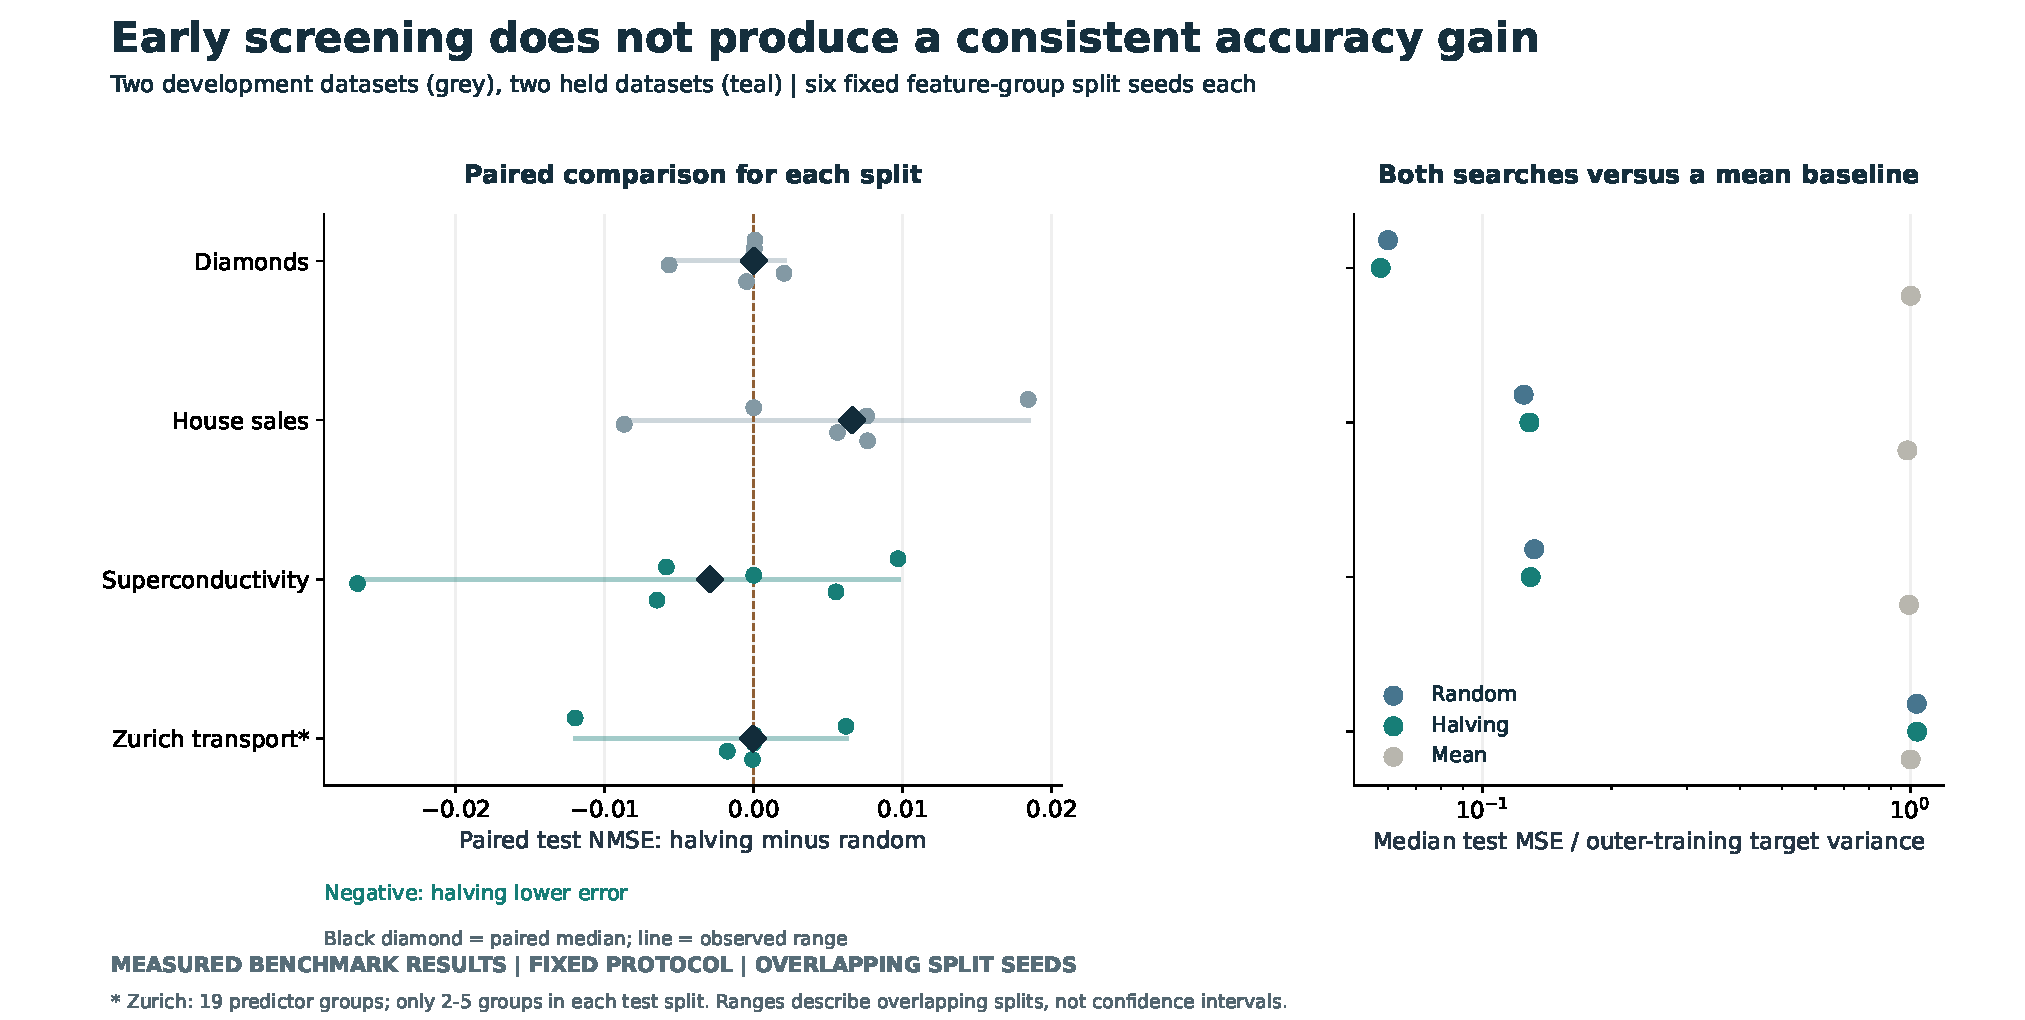
\includegraphics[width=.98\linewidth,height=.85\textheight,keepaspectratio]{images/paired-test-loss.pdf}
\par\small Figure 1. Paired split differences remain distinct from marginal medians. Ranges are descriptive, and the small Zurich group support is explicit.
\end{landscape}
\clearpage\begin{landscape}\centering
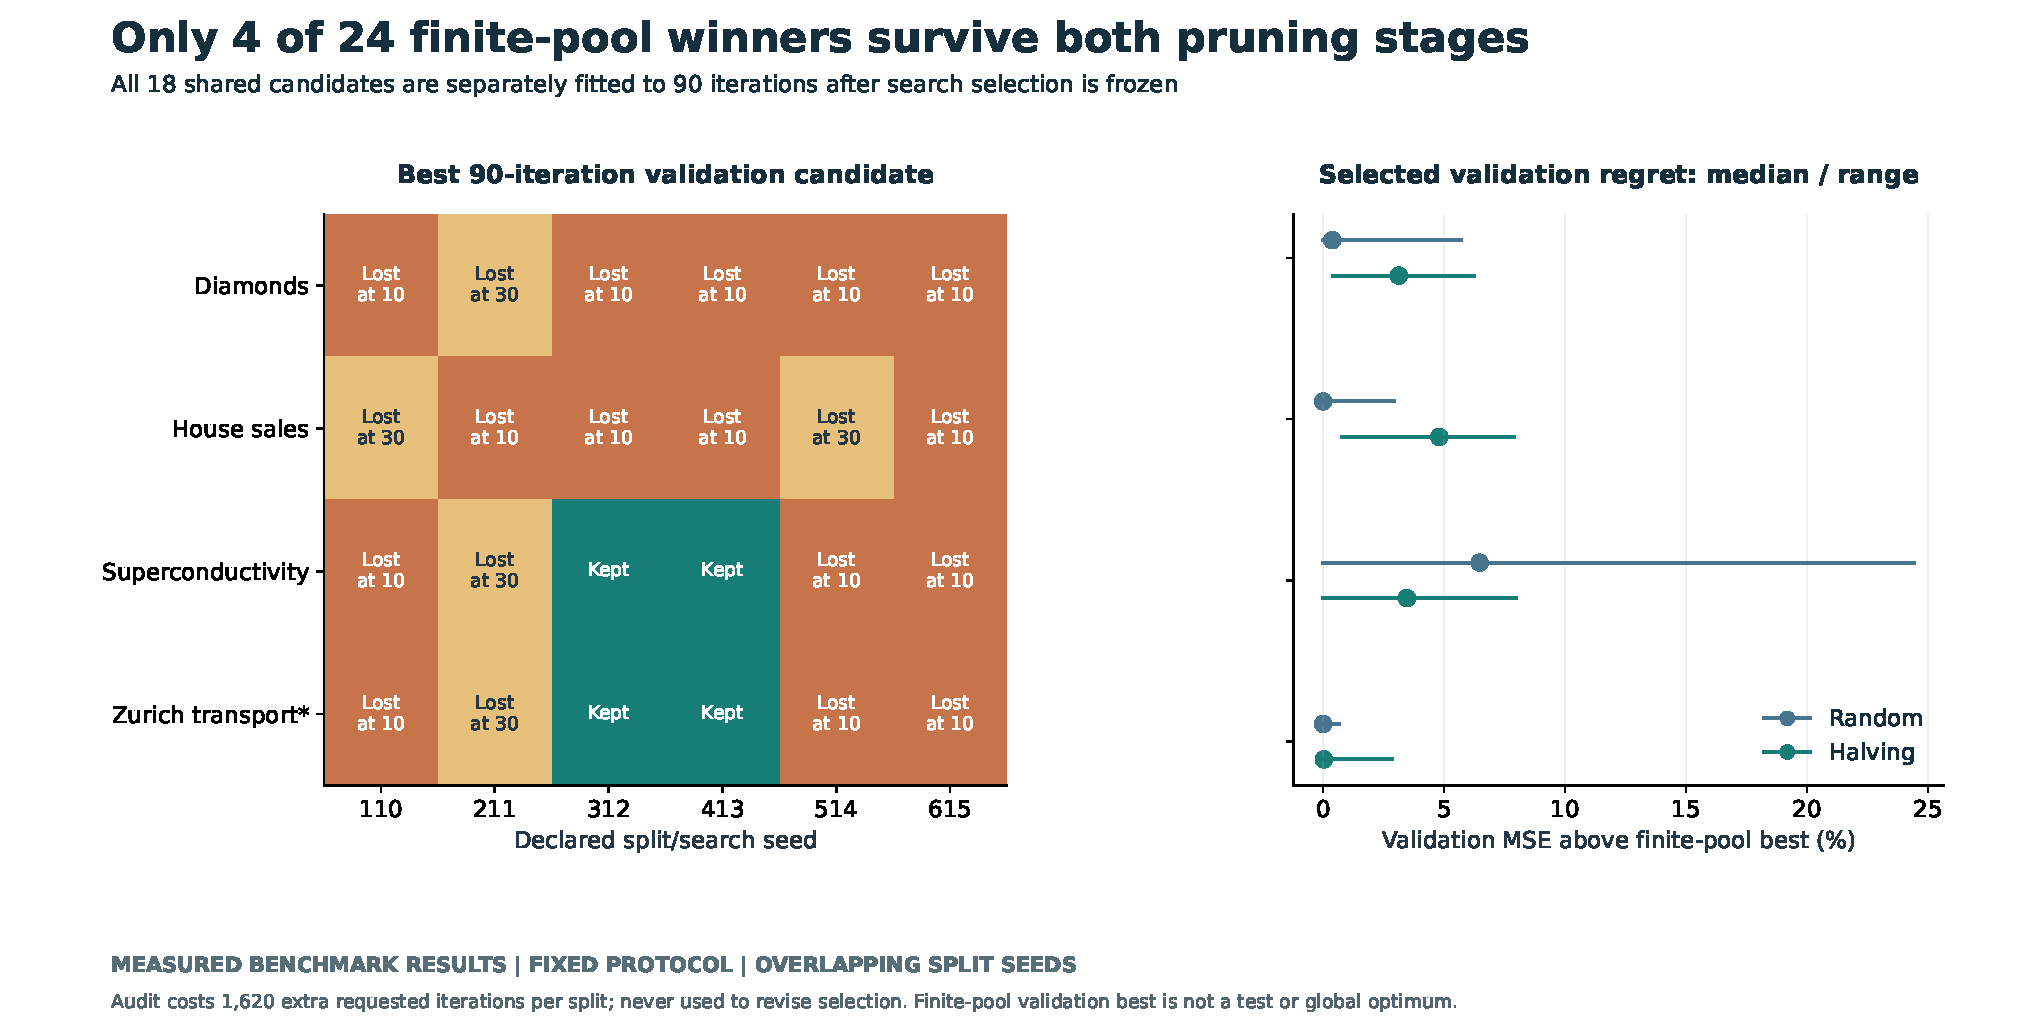
\includegraphics[width=.98\linewidth,height=.85\textheight,keepaspectratio]{images/early-elimination-audit.pdf}
\par\small Figure 2. A separately charged full-pool audit measures which validation winner early pruning discarded. It never changes the frozen selected model.
\end{landscape}
\clearpage\begin{landscape}\centering
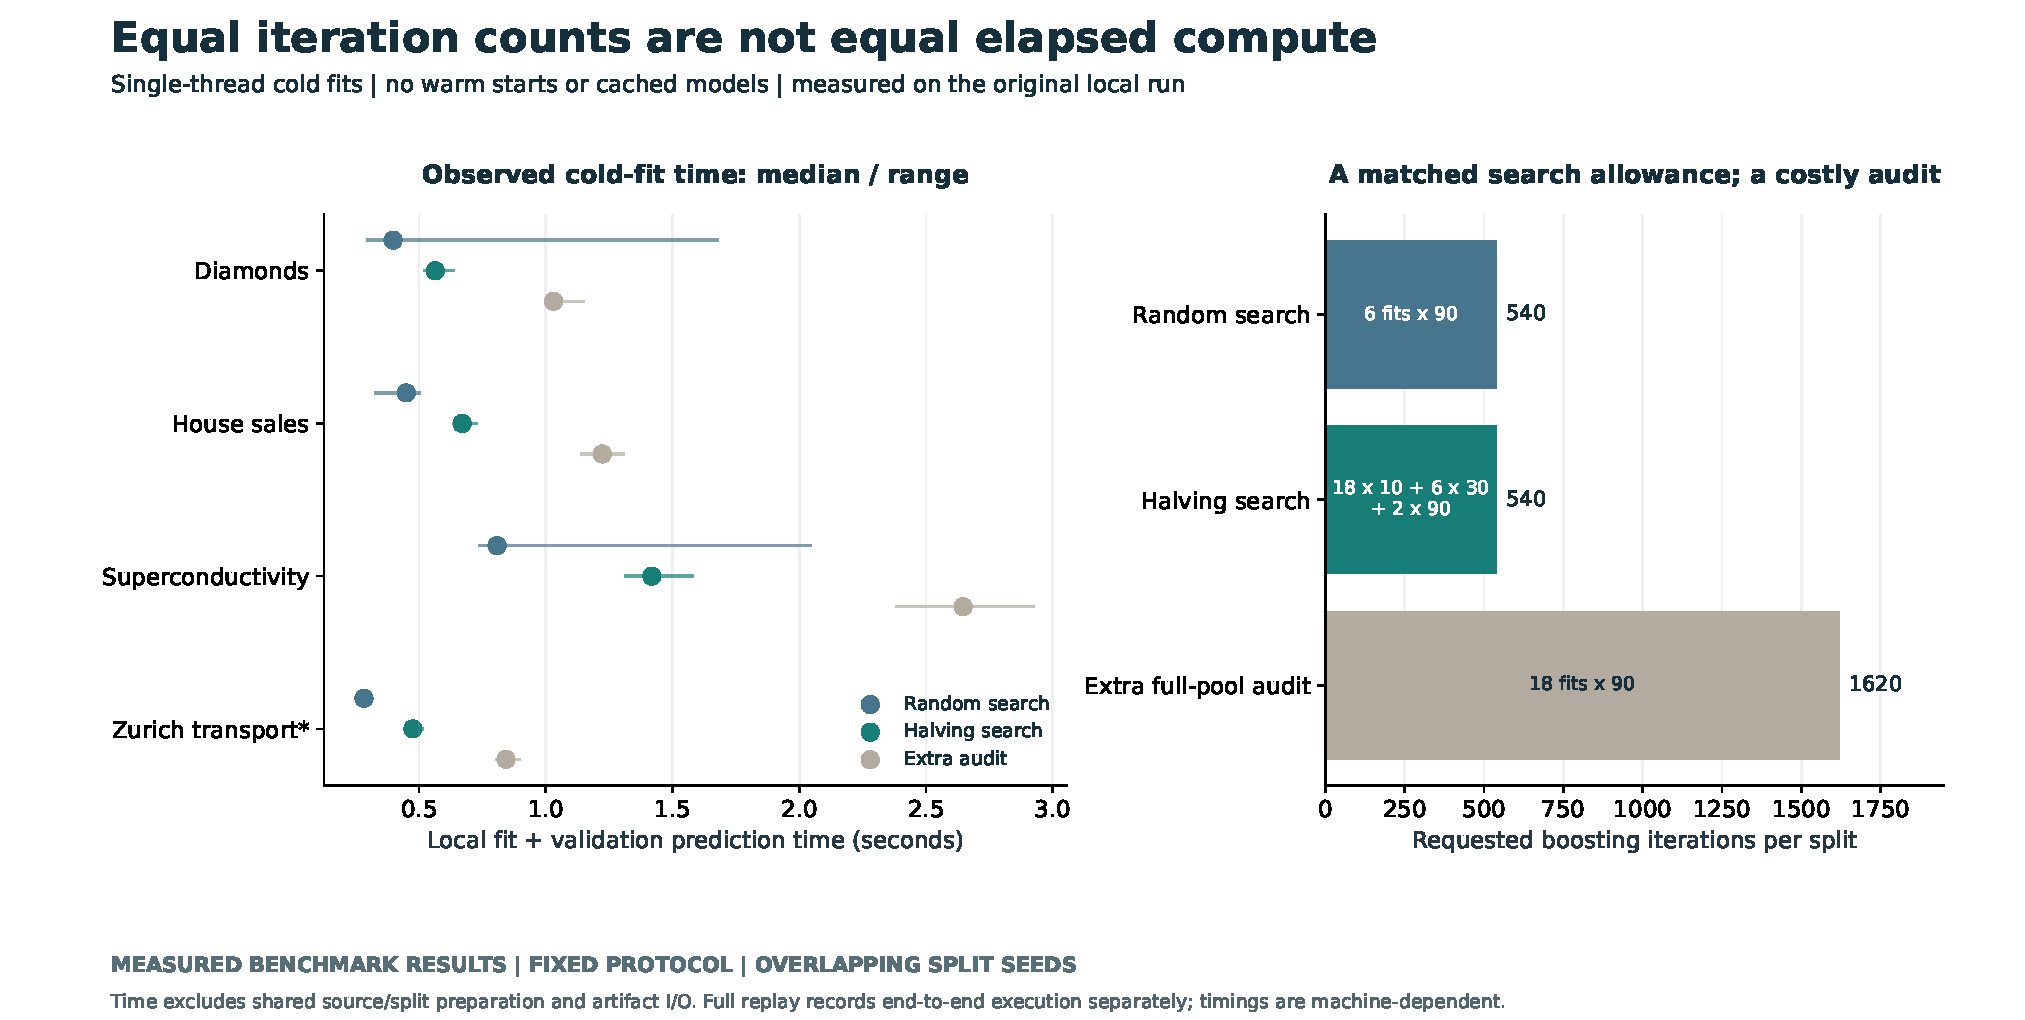
\includegraphics[width=.98\linewidth,height=.85\textheight,keepaspectratio]{images/resource-accounting.pdf}
\par\small Figure 3. Requested iterations match for the two searches, while measured cold-fit times differ. Research audit cost and timing scope remain visible.
\end{landscape}
\end{document}
